\subsection{Subpaso 1-A: Agregar Sala}
	Para agregar una sala a lo que se conoce como catálogo o a nuestro listado,
	se mostrará la interfaz \par
		\begin{figure}[hbtp]	
			\centering
				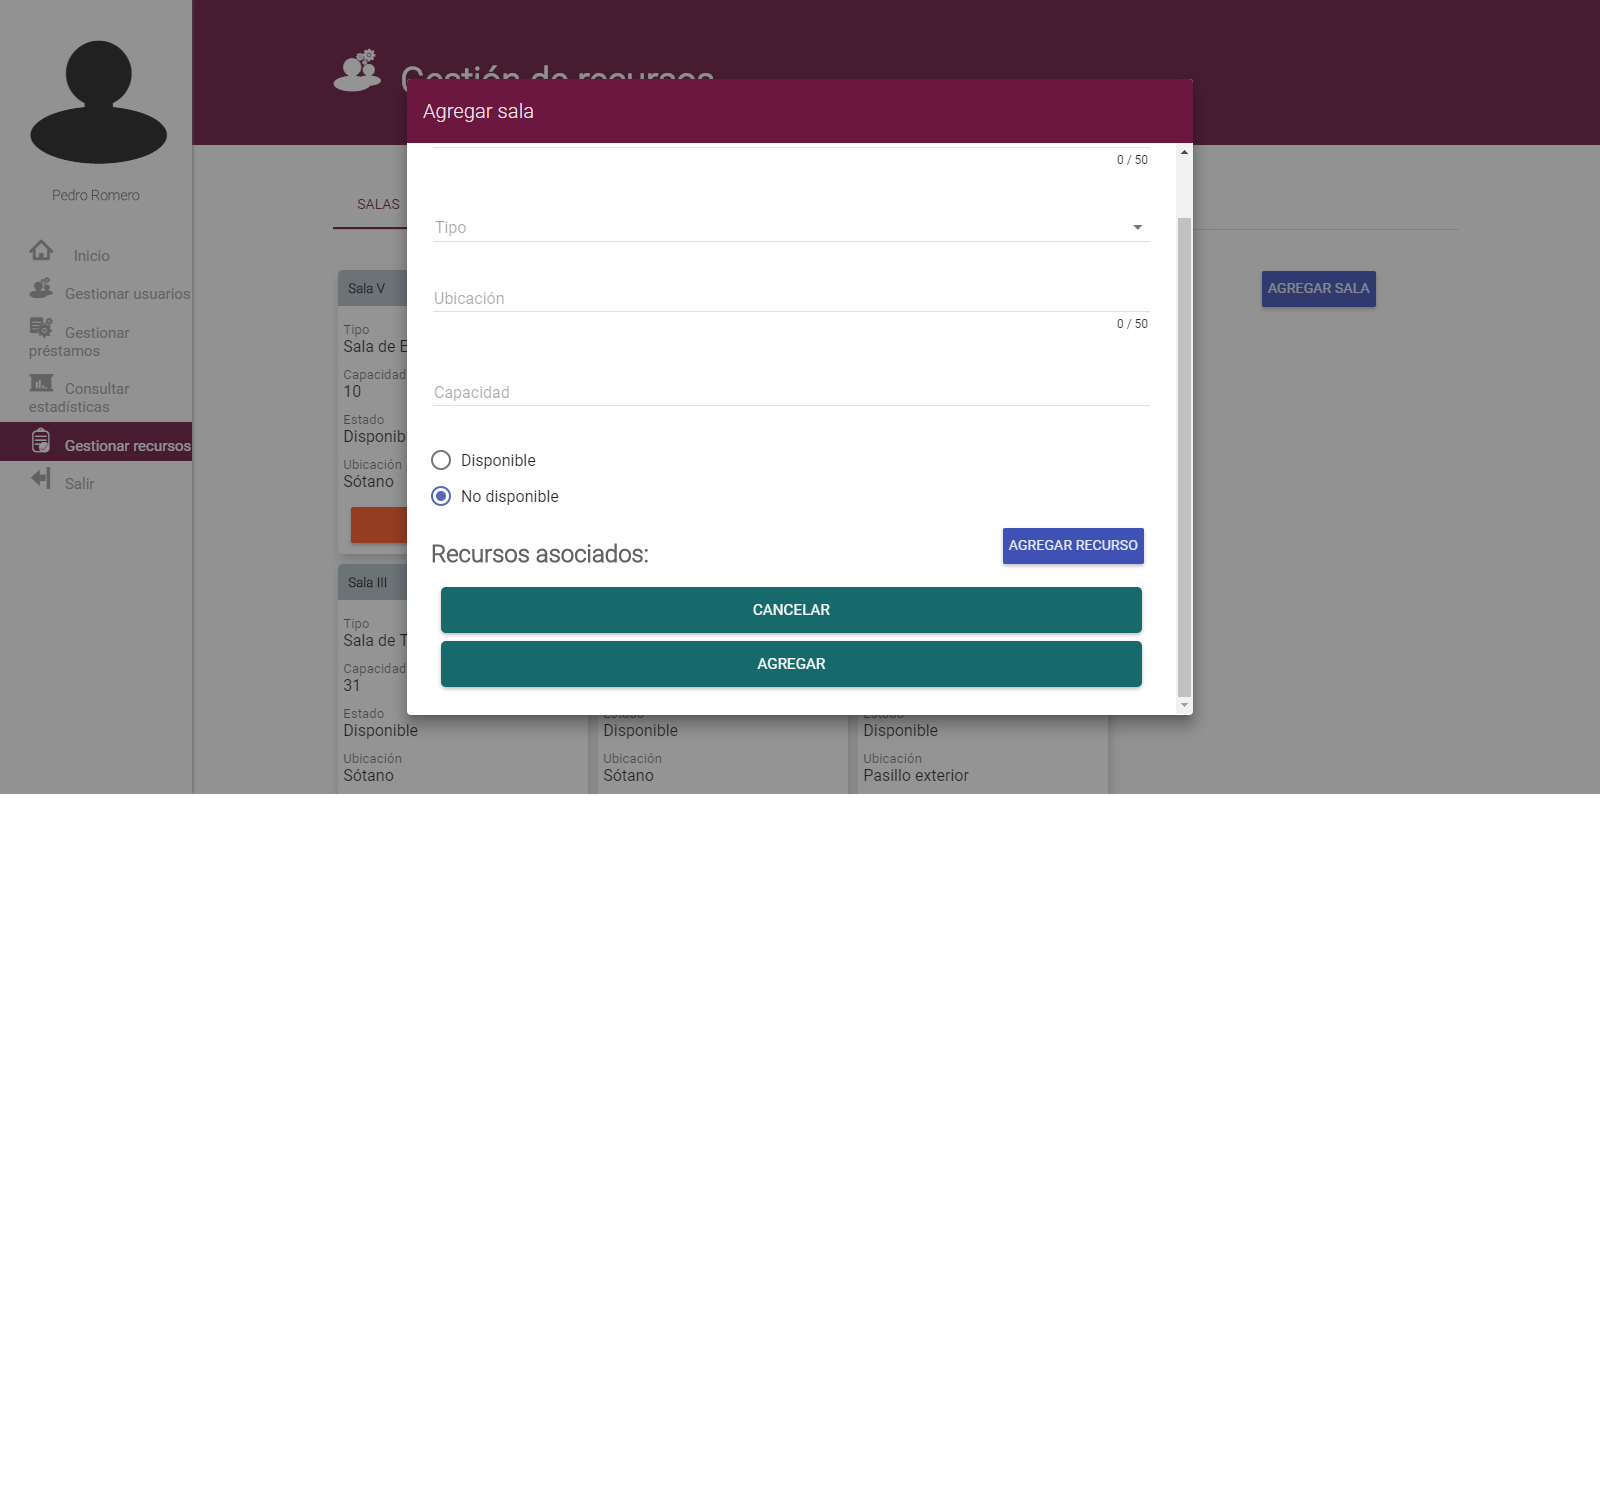
\includegraphics[scale=0.3]{images/Interfaz/IUGS38_AgregarSala.png}
				\caption{IUGS-38 Agregar una sala}
		\end{figure}
	
	\begin{enumerate}
		\item ingresa el nombre de la sala a crear.
		\item selecciona el tipo de sala a crear, tomandose en cuenta la capacidad
			que tendrá cada sala, como son:
			\begin{enumerate}
				\item Salas de estudio: 4 personas.
				\item Salas de trabajo: 15 personas.
				\item Salas de proyección: 20 personas.
			\end{enumerate}
		\item ingresa la ubicación.
		\item ingresa la capacidad.
		\item selecciona el estado de la nueva sala. 		
	\end{enumerate}
	
	Para concluir con la sala creada 
	\begin{enumerate}
		\item se presiona el botón \textbf{Agregar}
				de la misma interfaz. (Veáse error ER01).\par		
		 	\begin{figure}[hbtp]	
				\centering
					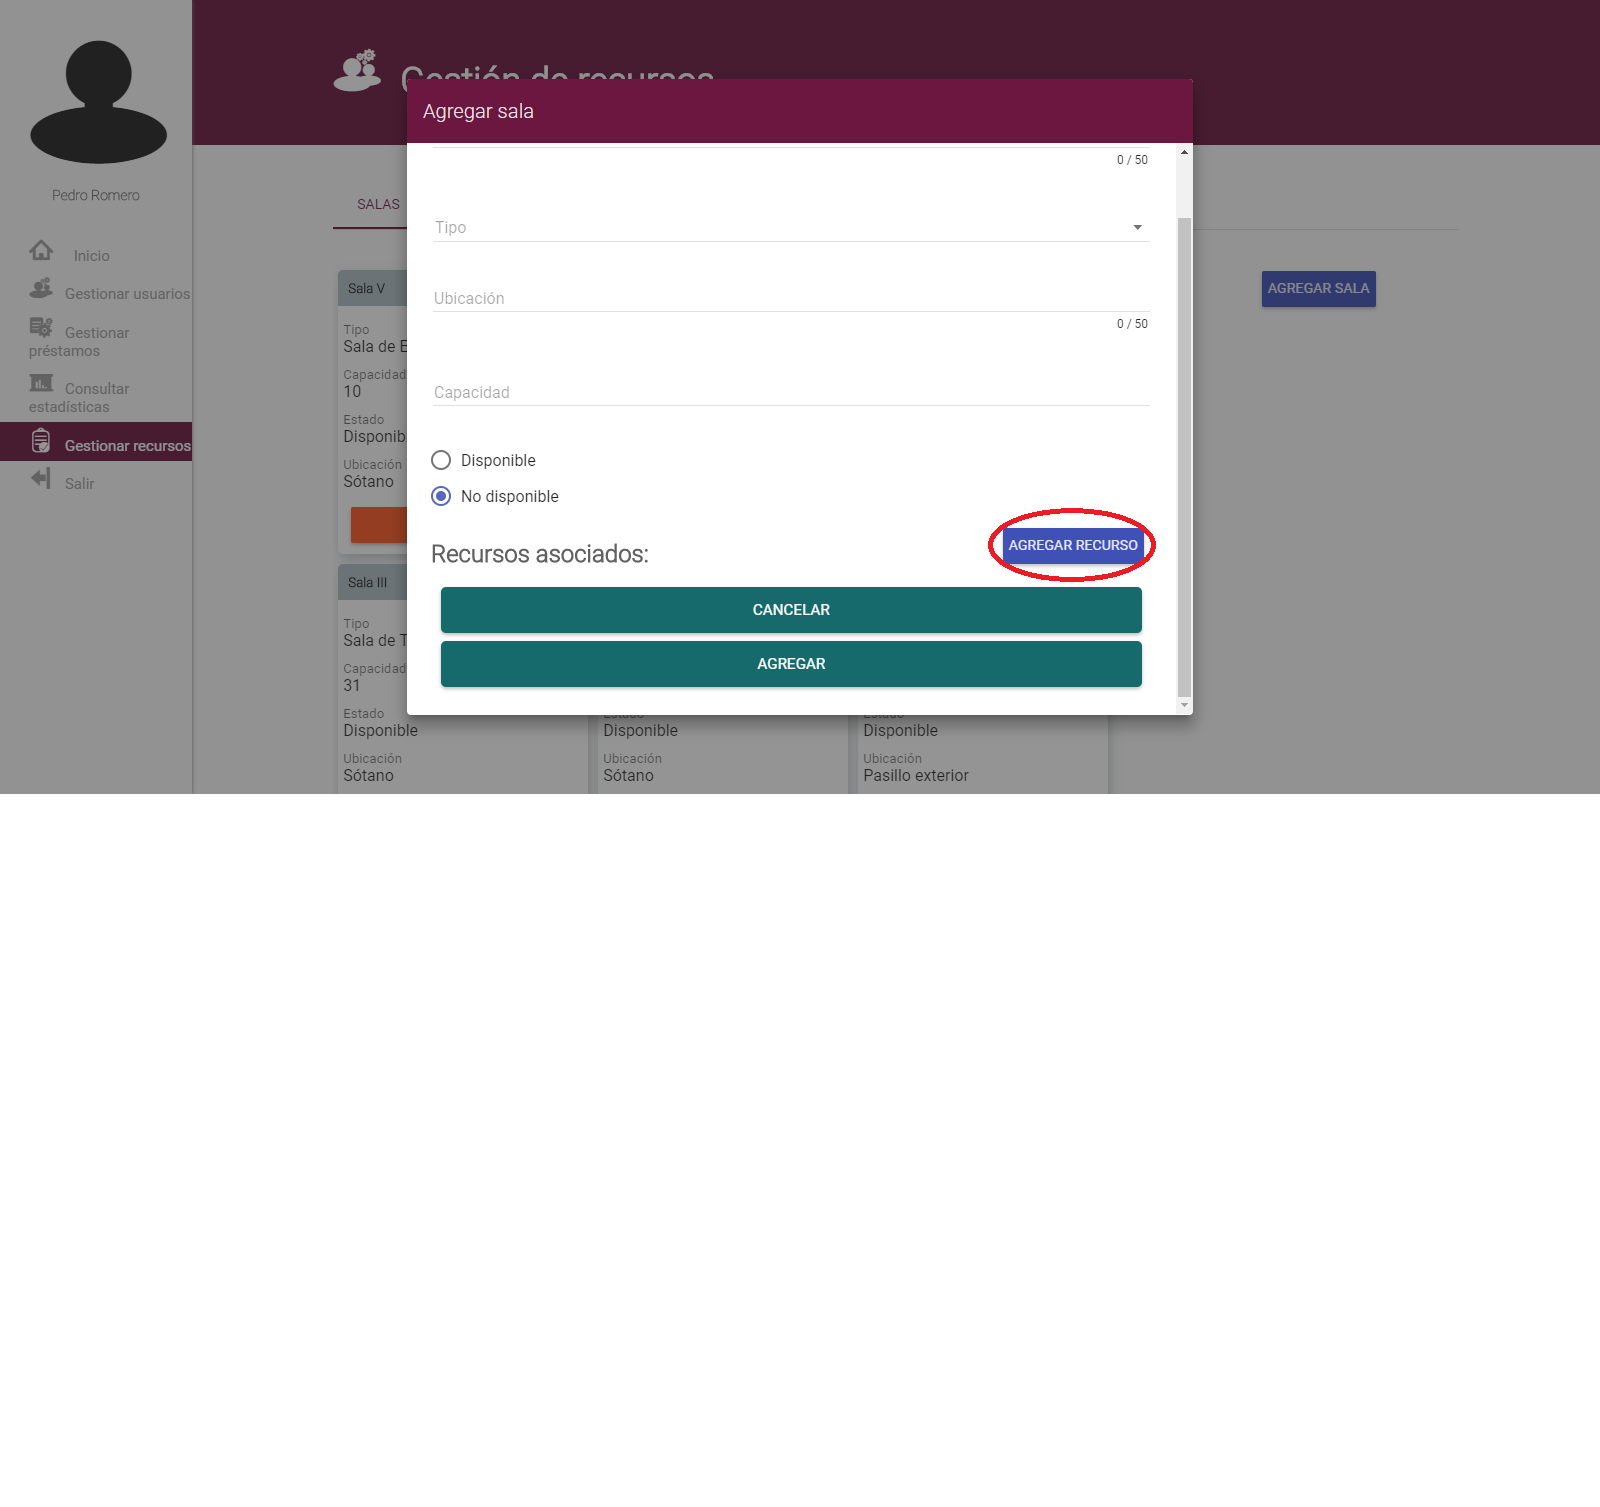
\includegraphics[scale=0.3]{images/Interfaz/IUGS38_AgregarSalaB.png}
					\caption{IUGS-38 Agregar una sala botón}
			\end{figure}
			
		\item Cuando todo se haya registrado correctamente, se mostrará 
			un mensaje \textit{El registro del nuevo recurso ha sido exitoso.}	
		\item se mostrará la interfaz \par
			\begin{figure}[hbtp]	
				\centering
					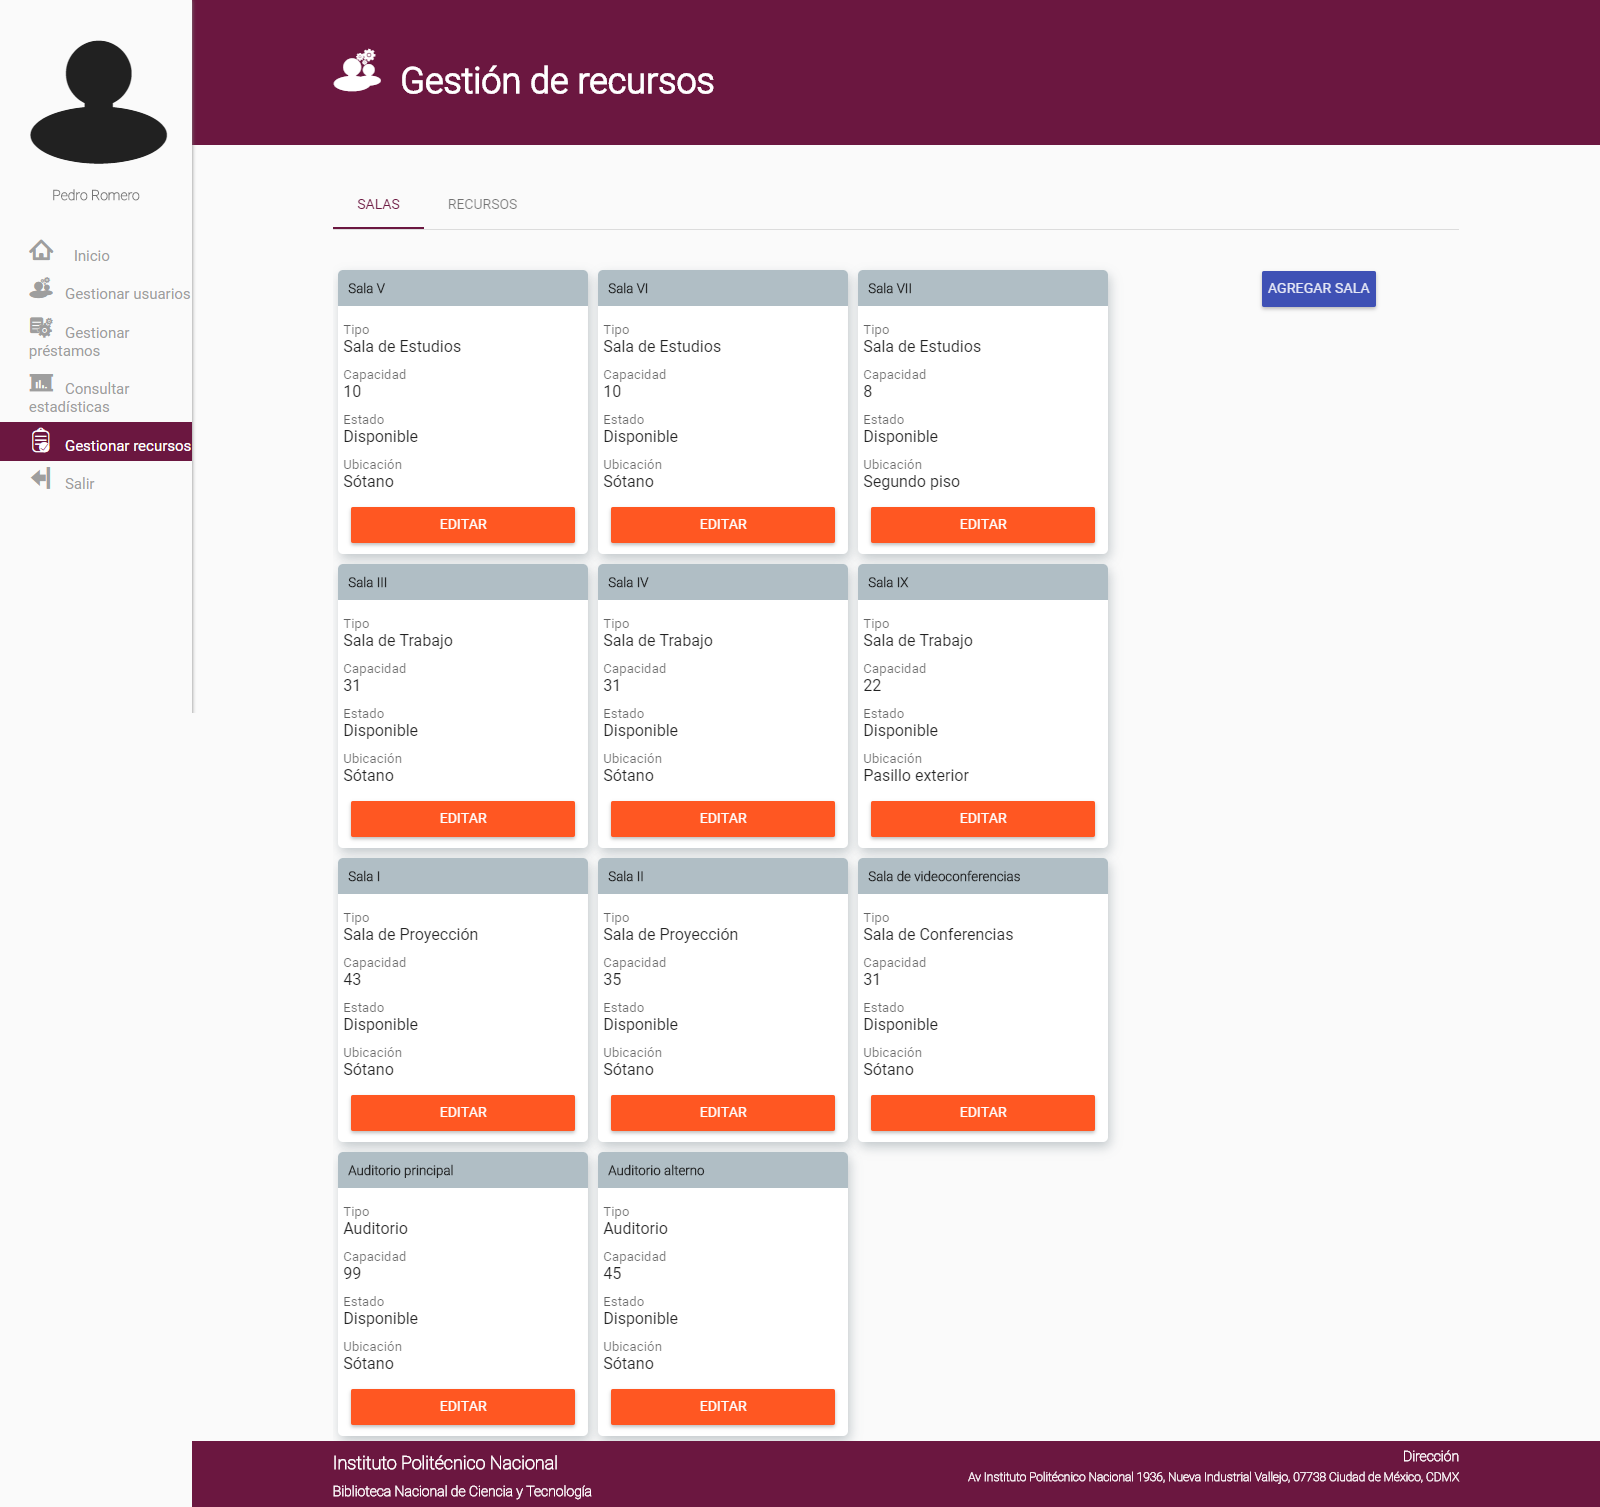
\includegraphics[scale=0.3]{images/Interfaz/IUGS21_GestionarRecursos.png}
					\caption{IUGS-21 Gestionar recursos}
			\end{figure}
	\end{enumerate}		

\textbf{Observación:} para cancelar el regitro del nuevo recurso
		\begin{enumerate}
			\item se presiona el botón \textbf{cancelar} de la interfaz
				\textbf{IUGS-38 Agregar una sala} 
			\item se mostrará la interfaz 	
				\textbf{IUGS-21 Gestionar recursos}
		\end{enumerate}
		
\subsection{Subpaso 2-B: agregar un nuevo subrecurso}
	para mostrar una nueva fila en la lista de sobrerecurso se realizará:	
	\begin{enumerate}
		\item El administrador de apoyo tecnico presiona el botón 
			\textbf{Agregar Recurso} que se encuentra en la parte inferior izquiera. \par
			\begin{figure}[hbtp]	
				\centering
					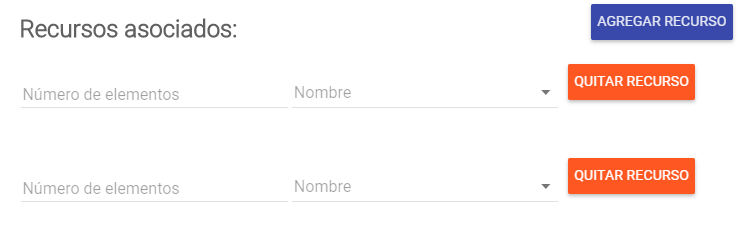
\includegraphics[scale=0.3]{images/Interfaz/IUGS37_Subrecurso.png}
					\caption{IUGS-37 subrecurso}
			\end{figure}
		\item el admnistrador selecciona el nuevo sobrecurso.
		\item \textit{se tomará en encuenta el sobrecurso con base en
			las existencias que hay sin analizar a otro recurso, de ser
			un caso positivo, se habilitará la entrada de cantidad}
		\item  el administrador ingresa el número de nuevos subrecursos.
		
	\end{enumerate}		
	
	
\subsection{Subpaso 3-B: quitar subrecurso}
	para eliminar una fila en la lista de sobrerecurso se realizará:	
	\begin{enumerate}
		\item El administrador de apoyo tecnico presiona el botón 
			\textbf{Quitar recurso} que se encuentra en la parte inferior derecha.
			\textbf{Agregar Recurso} que se encuentra en la parte inferior izquiera. \par
			\begin{figure}[hbtp]	
				\centering
					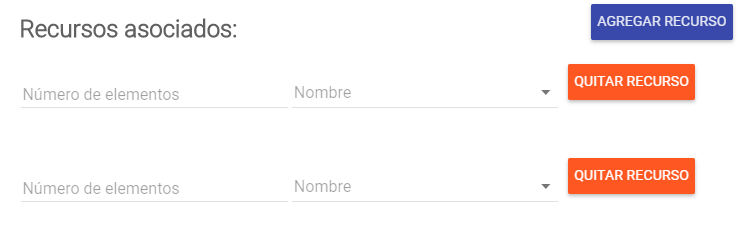
\includegraphics[scale=0.3]{images/Interfaz/IUGS37_Subrecurso.png}
					\caption{IUGS-37 subrecurso}
			\end{figure}
	\end{enumerate}		



\subsection{Subpaso 4-C: Error ERO1}
	Cuando los campos no hayan sido llenados correctamente
	se mostrará el siguiente mensaje \par	
	\textit{Este campo es requerido. }\par
	Se deberán ingresar todos los campos para continuar con agregar la sala.